%====================================================================
% Chapitre 4 : Conception du framework SecureIoT-VIF
%====================================================================

\chapter{Conception du framework SecureIoT-VIF}
\label{chap:framework-design}

\section{Introduction}

Ce chapitre présente la conception détaillée de SecureIoT-VIF (Secure IoT Verification Integrity Framework), notre solution de vérification d'intégrité pour les firmwares IoT basée sur les éléments sécurisés et modules de sécurité matérielle embarqués. La conception s'appuie sur l'analyse des menaces du chapitre précédent et intègre les meilleures pratiques identifiées dans l'état de l'art. Nous détaillons l'architecture globale, les composants principaux, les protocoles de sécurité, et les mécanismes d'optimisation développés pour respecter les contraintes des dispositifs IoT grand public.

\section{Architecture globale}

\subsection{Principes de conception}

La conception de SecureIoT-VIF repose sur plusieurs principes fondamentaux qui guident les choix architecturaux et techniques :

\textbf{Principe de sécurité par conception (Security by Design) :} Tous les composants du framework intègrent des mécanismes de sécurité dès leur conception, plutôt que de les ajouter comme des couches supplémentaires. Cette approche garantit une sécurité robuste sans compromettre les performances.

\textbf{Principe de défense en profondeur :} SecureIoT-VIF implémente plusieurs couches de sécurité complémentaires : vérification d'intégrité au démarrage, monitoring continu en temps réel, attestation à distance, et détection d'anomalies comportementales.

\textbf{Principe d'optimisation contrainte :} Chaque composant est optimisé pour fonctionner efficacement dans des environnements à ressources limitées, avec des mécanismes d'adaptation dynamique aux capacités disponibles.

\textbf{Principe de transparence opérationnelle :} Le framework fonctionne de manière transparente pour les applications utilisateur, minimisant l'impact sur les fonctionnalités normales du dispositif.

\subsection{Vue d'ensemble architecturale}

L'architecture de SecureIoT-VIF suit un modèle hiérarchique à quatre couches, chacune ayant des responsabilités spécifiques et interagissant avec les couches adjacentes selon des interfaces bien définies.

\begin{figure}[h]
    \centering
    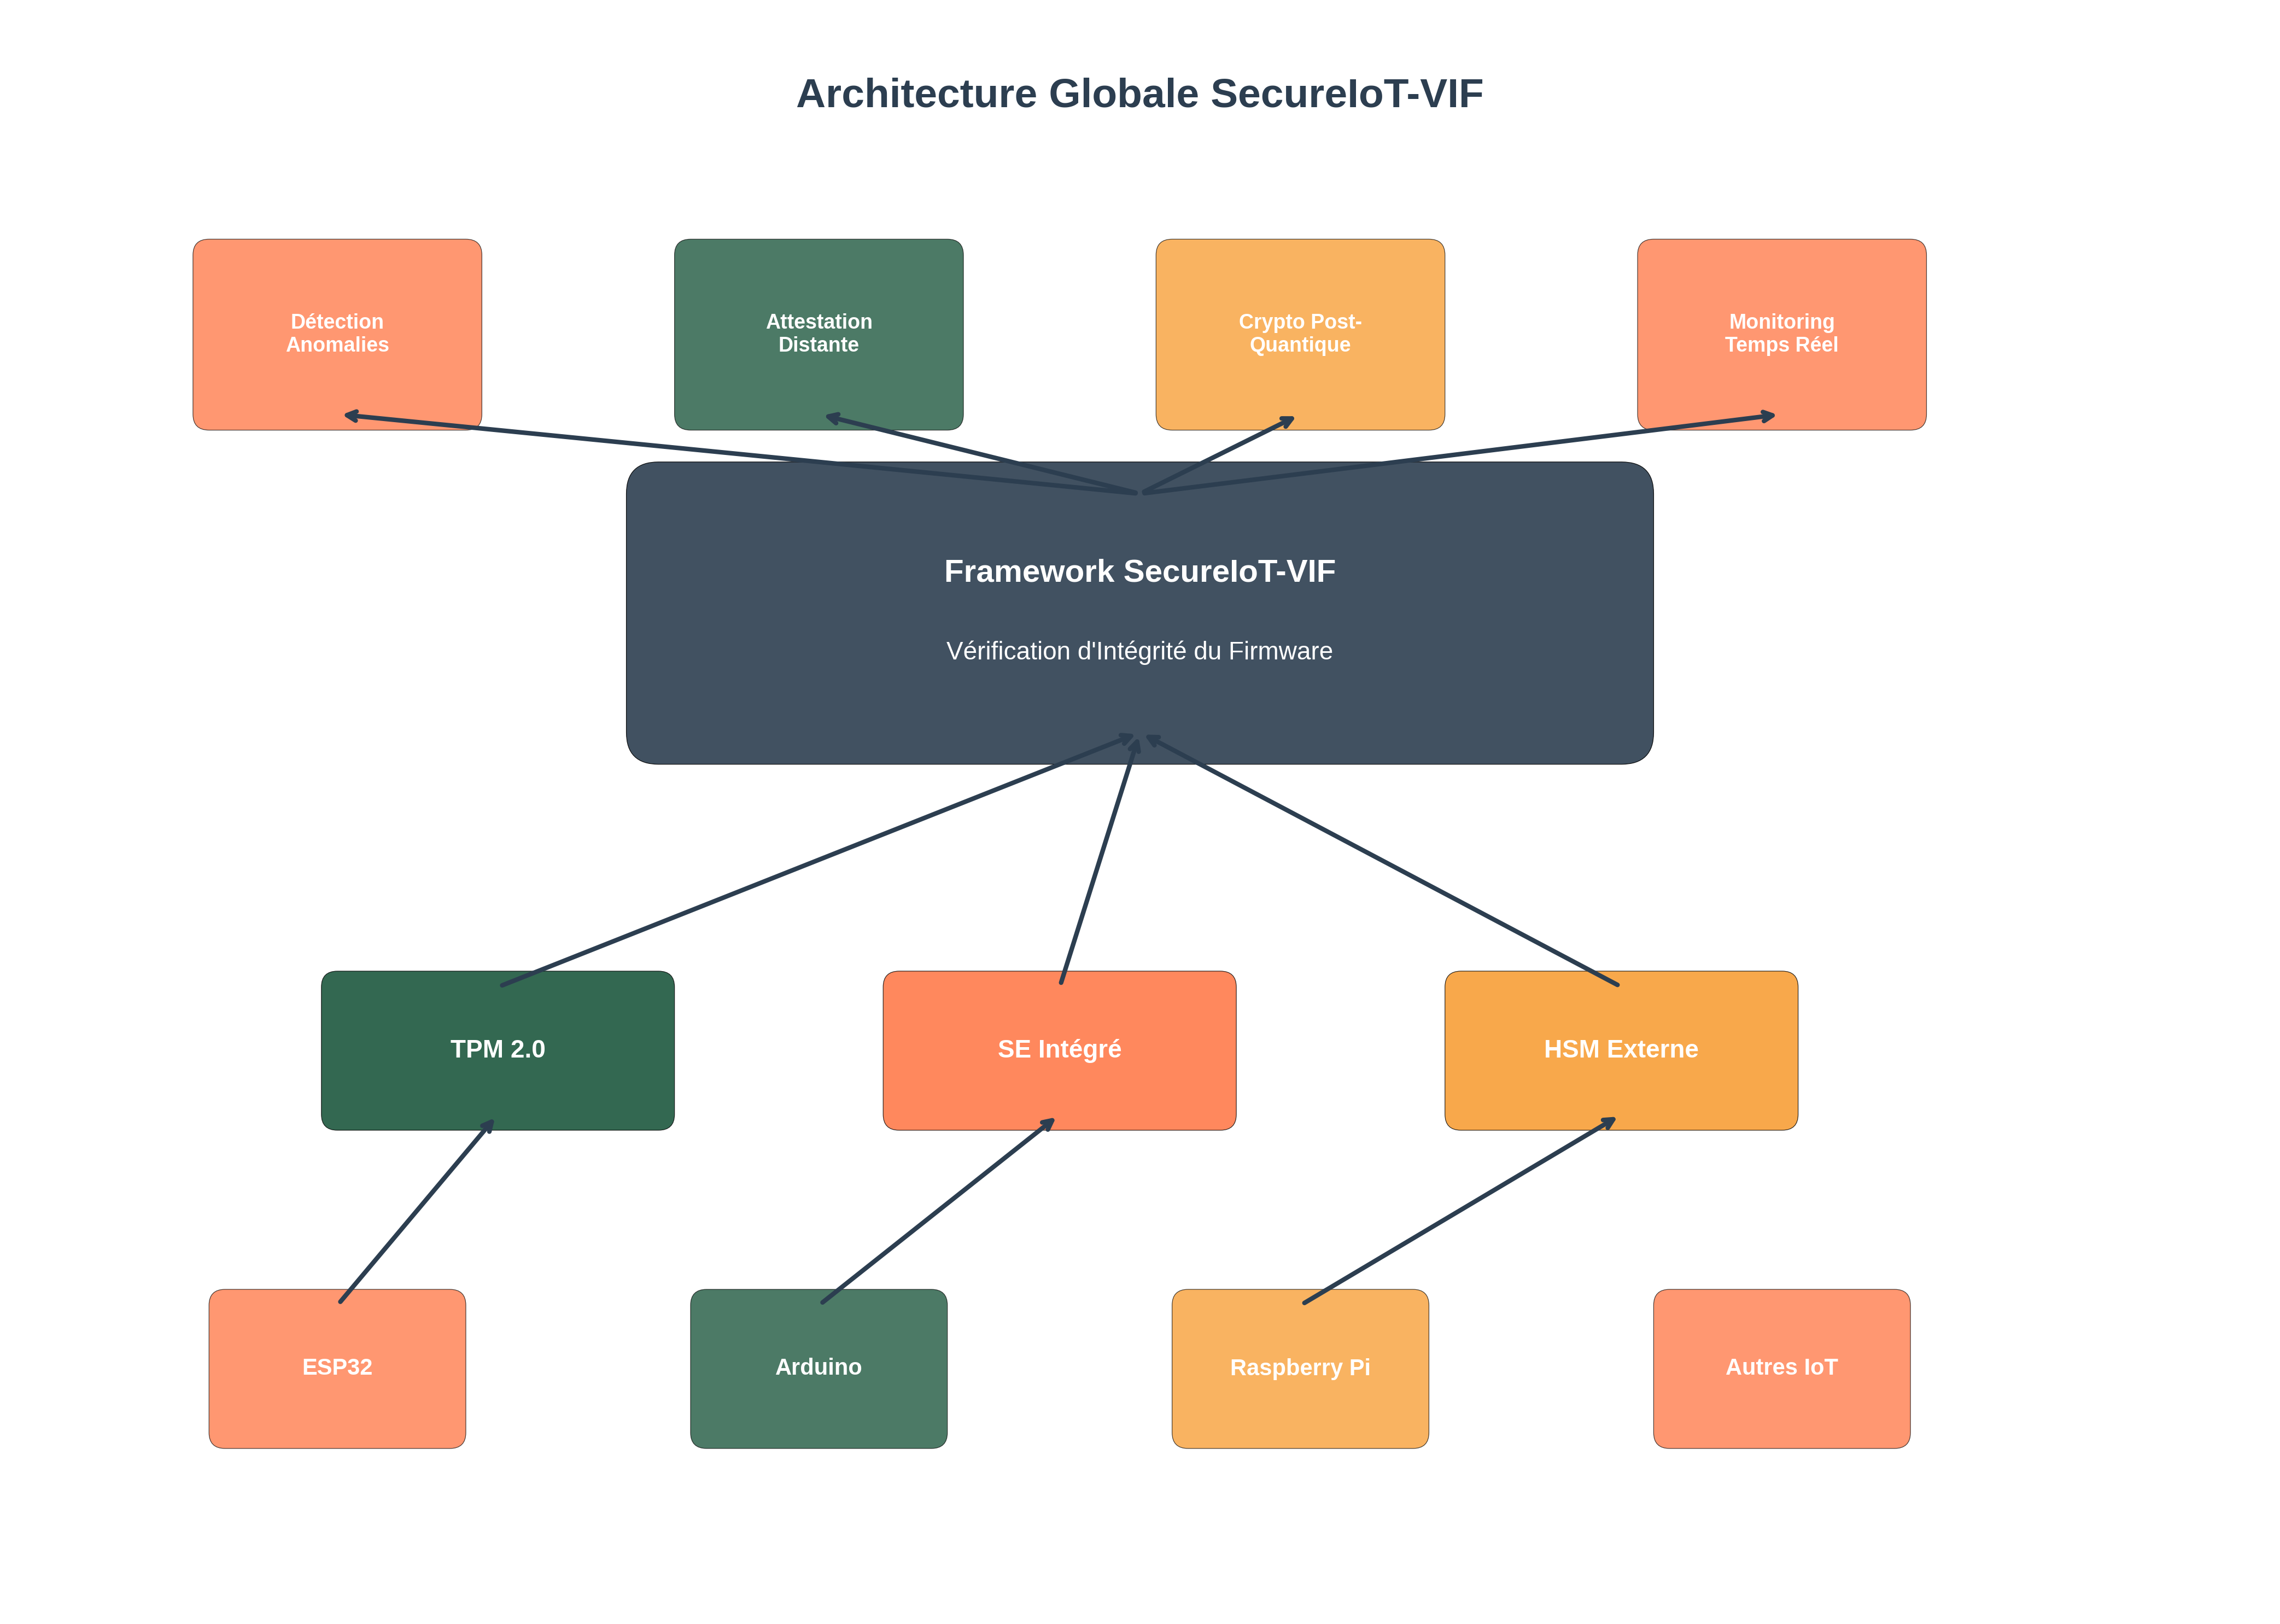
\includegraphics[width=0.9\textwidth]{assets/figures/secureiot_architecture.png}
    \caption{Architecture globale de SecureIoT-VIF}
    \label{fig:secureiot-architecture}
\end{figure}

\textbf{Couche matérielle sécurisée :} Cette couche fondamentale comprend les éléments sécurisés (\ac{SE}), modules de sécurité matérielle (\ac{HSM}), et autres composants cryptographiques matériels. Elle fournit les primitives de sécurité de base : génération de clés, calculs cryptographiques, stockage sécurisé, et attestation matérielle.

\textbf{Couche de vérification d'intégrité :} Cette couche implémente les mécanismes de vérification d'intégrité du firmware, incluant la vérification au démarrage (secure boot), le monitoring continu, et la détection de modifications. Elle s'appuie sur les services de la couche matérielle pour les opérations cryptographiques.

\textbf{Couche de services de sécurité :} Cette couche fournit les services de sécurité de haut niveau : attestation à distance, gestion des clés, détection d'anomalies, et réponse aux incidents. Elle orchestre les interactions entre les différents composants de sécurité.

\textbf{Couche d'interface applicative :} Cette couche expose les services de sécurité aux applications utilisateur et aux systèmes de gestion externe via des API standardisées. Elle assure la compatibilité avec les écosystèmes IoT existants.

\section{Composants principaux}

\subsection{Module de vérification d'intégrité (IVM)}

Le Module de Vérification d'Intégrité constitue le cœur de SecureIoT-VIF. Il implémente les mécanismes de vérification cryptographique de l'intégrité du firmware à différents moments du cycle de vie du dispositif.

\subsubsection{Vérification au démarrage (Secure Boot)}

Le processus de démarrage sécurisé établit une chaîne de confiance depuis la racine de confiance matérielle jusqu'au firmware applicatif. Cette approche s'inspire des travaux de Dave et al. \cite{Dave2023FVCARE} sur la vérification formelle des primitives de sécurité.

\textbf{Étape 1 - Initialisation de la racine de confiance :} Le processus démarre par l'activation de la racine de confiance matérielle, généralement implémentée dans une mémoire ROM immutable ou un élément sécurisé. Cette racine contient les clés publiques de vérification et les algorithmes cryptographiques de base.

\textbf{Étape 2 - Vérification du bootloader :} Le bootloader principal est vérifié cryptographiquement avant son exécution. Cette vérification utilise des signatures numériques basées sur ECDSA ou Ed25519 pour minimiser l'overhead computationnel.

\textbf{Étape 3 - Vérification du kernel :} Le kernel du système d'exploitation embarqué est vérifié selon le même processus, établissant une chaîne de confiance continue.

\textbf{Étape 4 - Vérification du firmware applicatif :} Le firmware applicatif principal est vérifié et son intégrité est attestée avant le démarrage des services utilisateur.

\subsubsection{Vérification continue (Runtime Verification)}

Contrairement aux approches traditionnelles qui ne vérifient l'intégrité qu'au démarrage, SecureIoT-VIF implémente une vérification continue pendant l'exécution. Cette approche s'inspire des travaux de Noor et al. \cite{Noor2025EILID} sur la surveillance continue de l'intégrité d'exécution.

\textbf{Mécanisme de hachage incrémental :} Le firmware est divisé en blocs de taille fixe (typiquement 4 KB) et chaque bloc est haché périodiquement. Cette approche permet de détecter les modifications localisées sans recalculer l'intégrité complète.

\textbf{Vérification basée sur les événements :} Certains événements système (chargement de modules, modifications de mémoire critique) déclenchent automatiquement des vérifications d'intégrité ciblées.

\textbf{Optimisation temporelle :} La vérification continue utilise des algorithmes d'ordonnancement adaptatifs pour minimiser l'impact sur les performances tout en maintenant une couverture de sécurité maximale.

\subsection{Module d'attestation à distance (RAM)}

Le Module d'Attestation à Distance permet aux dispositifs IoT de prouver leur intégrité à des vérificateurs distants sans compromettre la sécurité locale. L'implémentation s'inspire des protocoles développés par Kohli et al. \cite{Kohli2024SwarmNet} pour l'attestation dans les essaims IoT.

\subsubsection{Protocole d'attestation léger}

Le protocole d'attestation de SecureIoT-VIF est optimisé pour les environnements IoT contraints :

\textbf{Phase 1 - Génération de la preuve :} Le dispositif génère une preuve cryptographique de son état actuel, incluant les hash des composants critiques du firmware et les métadonnées d'exécution.

\textbf{Phase 2 - Signature de la preuve :} La preuve est signée cryptographiquement en utilisant des clés stockées dans l'élément sécurisé. La signature utilise des schémas légers comme Ed25519 ou les signatures basées sur hash (SPHINCS+).

\textbf{Phase 3 - Transmission sécurisée :} La preuve signée est transmise au vérificateur via un canal sécurisé, typiquement TLS 1.3 avec des suites cryptographiques optimisées.

\textbf{Phase 4 - Vérification distante :} Le vérificateur valide la signature et compare la preuve avec les valeurs de référence attendues.

\subsubsection{Optimisations pour l'IoT}

\textbf{Attestation par lots :} Plusieurs dispositifs peuvent être attestés simultanément en utilisant des techniques de signature par lots, réduisant l'overhead de communication.

\textbf{Attestation différée :} Pour les dispositifs avec des connexions intermittentes, l'attestation peut être différée et agrégée lors de la reconnexion.

\textbf{Compression des preuves :} Les preuves d'attestation utilisent des techniques de compression spécialisées pour minimiser la taille des messages.

\subsection{Module de détection d'anomalies (ADM)}

Le Module de Détection d'Anomalies implémente des techniques d'apprentissage automatique pour identifier les comportements anormaux sans nécessiter de signatures d'attaques connues. L'approche s'inspire des travaux d'Alrawi et al. \cite{Alrawi2023MachineLearning} sur la détection de malwares par analyse de flot de contrôle.

\subsubsection{Collecte de métriques comportementales}

\textbf{Métriques de flot de contrôle :} Analyse des patterns d'exécution, fréquence des appels système, et séquences d'instructions pour détecter les déviations du comportement normal.

\textbf{Métriques de ressources :} Surveillance de l'utilisation CPU, mémoire, et réseau pour identifier les consommations anormales indicatrices d'activité malveillante.

\textbf{Métriques de communication :} Analyse des patterns de communication réseau pour détecter les communications avec des serveurs de commande et contrôle.

\subsubsection{Algorithmes de détection}

\textbf{Apprentissage non supervisé :} Utilisation d'algorithmes de clustering (K-means, DBSCAN) pour identifier les patterns normaux et détecter les déviations.

\textbf{Réseaux de neurones légers :} Implémentation de réseaux de neurones optimisés pour les environnements contraints, capables de fonctionner avec moins de 32 KB de mémoire.

\textbf{Analyse temporelle :} Prise en compte de la dimension temporelle dans l'analyse des comportements pour détecter les attaques sophistiquées.

\subsection{Module de gestion des clés (KMM)}

Le Module de Gestion des Clés assure la génération, le stockage, la distribution, et la révocation des clés cryptographiques utilisées par SecureIoT-VIF.

\subsubsection{Hiérarchie des clés}

\textbf{Clé racine (Root Key) :} Stockée dans l'élément sécurisé, cette clé ne quitte jamais le dispositif et sert à dériver les autres clés.

\textbf{Clés d'intégrité :} Utilisées pour les calculs de hash et la vérification d'intégrité, dérivées de la clé racine.

\textbf{Clés d'attestation :} Utilisées pour signer les preuves d'attestation, renouvelées périodiquement.

\textbf{Clés de communication :} Utilisées pour les communications sécurisées, gérées selon les protocoles de gestion de clés standard.

\subsubsection{Protocoles de gestion}

\textbf{Génération sécurisée :} Utilisation de générateurs de nombres aléatoires matériels pour assurer l'entropie des clés.

\textbf{Stockage sécurisé :} Les clés sensibles sont stockées exclusivement dans les éléments sécurisés avec protection contre l'extraction.

\textbf{Rotation automatique :} Mécanisme de rotation périodique des clés pour limiter l'impact d'une compromission.

\textbf{Révocation distribuée :} Système de révocation de clés compatible avec les environnements IoT distribués.

\section{Protocoles de sécurité}

\subsection{Protocole de démarrage sécurisé}

Le protocole de démarrage sécurisé de SecureIoT-VIF établit une chaîne de confiance robuste tout en minimisant l'impact sur le temps de démarrage. L'approche s'inspire des travaux de Parisi et al. \cite{Parisi2024TitanCFI} sur l'enforcement de l'intégrité du flot de contrôle dans la racine de confiance.

\begin{algorithm}
\caption{Protocole de démarrage sécurisé SecureIoT-VIF}
\label{alg:secure-boot}
\begin{algorithmic}[1]
\State \textbf{Initialisation}
\State $HSM \leftarrow$ Activer\_HSM()
\State $K_{root} \leftarrow$ Récupérer\_Clé\_Racine($HSM$)
\State $État \leftarrow$ INIT

\State \textbf{Vérification du bootloader}
\State $Signature_{BL} \leftarrow$ Lire\_Signature\_Bootloader()
\State $Hash_{BL} \leftarrow$ Calculer\_Hash\_Bootloader()
\If{Vérifier\_Signature($Hash_{BL}$, $Signature_{BL}$, $K_{root}$)}
    \State $État \leftarrow$ BOOTLOADER\_VÉRIFIÉ
\Else
    \State Déclencher\_Alerte\_Sécurité()
    \State \textbf{return} ÉCHEC
\EndIf

\State \textbf{Vérification du kernel}
\State $Signature_{Kernel} \leftarrow$ Lire\_Signature\_Kernel()
\State $Hash_{Kernel} \leftarrow$ Calculer\_Hash\_Kernel()
\If{Vérifier\_Signature($Hash_{Kernel}$, $Signature_{Kernel}$, $K_{root}$)}
    \State $État \leftarrow$ KERNEL\_VÉRIFIÉ
\Else
    \State Déclencher\_Alerte\_Sécurité()
    \State \textbf{return} ÉCHEC
\EndIf

\State \textbf{Vérification du firmware applicatif}
\State $Signature_{App} \leftarrow$ Lire\_Signature\_Application()
\State $Hash_{App} \leftarrow$ Calculer\_Hash\_Application()
\If{Vérifier\_Signature($Hash_{App}$, $Signature_{App}$, $K_{root}$)}
    \State $État \leftarrow$ FIRMWARE\_VÉRIFIÉ
    \State Initialiser\_Monitoring\_Continu()
    \State \textbf{return} SUCCÈS
\Else
    \State Déclencher\_Alerte\_Sécurité()
    \State \textbf{return} ÉCHEC
\EndIf
\end{algorithmic}
\end{algorithm}

\subsection{Protocole de vérification continue}

La vérification continue représente une innovation majeure de SecureIoT-VIF, permettant la détection d'attaques pendant l'exécution du firmware.

\begin{algorithm}
\caption{Protocole de vérification continue}
\label{alg:continuous-verification}
\begin{algorithmic}[1]
\State \textbf{Initialisation}
\State $Blocs \leftarrow$ Diviser\_Firmware\_En\_Blocs()
\State $Hashes\_Référence \leftarrow$ Calculer\_Hashes\_Initiaux($Blocs$)
\State $Scheduler \leftarrow$ Initialiser\_Ordonnanceur()

\State \textbf{Boucle de vérification}
\While{$Dispositif\_Actif$}
    \State $Bloc\_Actuel \leftarrow$ Scheduler.Sélectionner\_Bloc\_Suivant()
    \State $Hash\_Actuel \leftarrow$ Calculer\_Hash($Bloc\_Actuel$)
    \State $Hash\_Référence \leftarrow$ Hashes\_Référence[$Bloc\_Actuel$]
    
    \If{$Hash\_Actuel \neq Hash\_Référence$}
        \State $Anomalie \leftarrow$ Analyser\_Modification($Bloc\_Actuel$)
        \If{$Anomalie$ == MALVEILLANTE}
            \State Déclencher\_Réponse\_Incident()
            \State Notifier\_Attestation\_Distante()
        \EndIf
    \EndIf
    
    \State Attendre\_Prochaine\_Vérification()
\EndWhile
\end{algorithmic}
\end{algorithm}

\subsection{Protocole d'attestation à distance}

Le protocole d'attestation à distance permet aux dispositifs IoT de prouver leur intégrité à des vérificateurs externes. L'implémentation optimise les communications pour les environnements contraints.

\begin{algorithm}
\caption{Protocole d'attestation à distance}
\label{alg:remote-attestation}
\begin{algorithmic}[1]
\State \textbf{Réception de la requête d'attestation}
\State $Requête \leftarrow$ Recevoir\_Requête\_Attestation()
\State $Nonce \leftarrow$ Extraire\_Nonce($Requête$)
\State $Challenge \leftarrow$ Extraire\_Challenge($Requête$)

\State \textbf{Génération de la preuve}
\State $Mesures \leftarrow$ Collecter\_Mesures\_Système()
\State $Preuve \leftarrow$ Construire\_Preuve($Mesures$, $Nonce$, $Challenge$)
\State $Signature \leftarrow$ Signer\_Preuve($Preuve$, $K_{attestation}$)

\State \textbf{Transmission de la réponse}
\State $Réponse \leftarrow$ Construire\_Réponse($Preuve$, $Signature$)
\State $Réponse\_Compressée \leftarrow$ Comprimer\_Réponse($Réponse$)
\State Transmettre\_Réponse($Réponse\_Compressée$)

\State \textbf{Gestion de la vérification}
\State $Résultat \leftarrow$ Attendre\_Résultat\_Vérification()
\If{$Résultat$ == ÉCHEC}
    \State Déclencher\_Procédure\_Récupération()
\EndIf
\end{algorithmic}
\end{algorithm}

\section{Mécanismes d'optimisation}

\subsection{Optimisations cryptographiques}

\subsubsection{Sélection d'algorithmes légers}

SecureIoT-VIF utilise des algorithmes cryptographiques spécifiquement optimisés pour les environnements contraints :

\textbf{Signatures numériques :} Ed25519 pour les signatures courtes et les vérifications rapides, SPHINCS+ pour la résistance post-quantique.

\textbf{Fonctions de hachage :} BLAKE2s pour les calculs d'intégrité, SHA-3 pour la compatibilité avec les standards existants.

\textbf{Chiffrement symétrique :} ChaCha20-Poly1305 pour les communications sécurisées, AES-GCM pour les données stockées.

\subsubsection{Optimisations matérielles}

\textbf{Accélération cryptographique :} Utilisation des accélérateurs cryptographiques intégrés dans les éléments sécurisés pour réduire l'overhead computationnel.

\textbf{Calculs parallèles :} Parallélisation des opérations cryptographiques sur les processeurs multi-cœurs disponibles.

\textbf{Optimisations mémoire :} Algorithmes de hachage en streaming pour minimiser l'utilisation de la RAM.

\subsection{Optimisations énergétiques}

\subsubsection{Gestion adaptative de la puissance}

\textbf{Ordonnancement adaptatif :} Ajustement dynamique de la fréquence de vérification en fonction de l'état de la batterie et de la charge système.

\textbf{Optimisation des communications :} Agrégation des messages d'attestation pour réduire le nombre de transmissions radio.

\textbf{Modes de veille intelligents :} Suspension des vérifications non critiques pendant les périodes de faible activité.

\subsubsection{Techniques de conservation d'énergie}

\textbf{Vérification différée :} Report des vérifications non urgentes aux périodes de charge de la batterie.

\textbf{Optimisation des algorithmes :} Utilisation d'algorithmes approximatifs pour les vérifications non critiques.

\textbf{Coopération énergétique :} Partage de la charge de vérification entre dispositifs dans les réseaux maillés.

\subsection{Optimisations de performance}

\subsubsection{Techniques de mise en cache}

\textbf{Cache de signatures :} Mise en cache des signatures vérifiées pour éviter les recalculs.

\textbf{Cache de hashes :} Stockage des hashes de blocs fréquemment vérifiés.

\textbf{Cache de métadonnées :} Mise en cache des informations d'attestation pour accélérer les requêtes.

\subsubsection{Parallélisation des opérations}

\textbf{Vérification parallèle :} Vérification simultanée de plusieurs blocs de firmware.

\textbf{Pipeline de traitement :} Chevauchement des phases de collecte, calcul, et vérification.

\textbf{Traitement distribué :} Répartition des calculs sur plusieurs processeurs disponibles.

\section{Adaptation aux contraintes IoT}

\subsection{Gestion des ressources limitées}

\subsubsection{Adaptation dynamique}

SecureIoT-VIF implémente des mécanismes d'adaptation dynamique pour fonctionner efficacement sur des dispositifs aux capacités variables :

\textbf{Profilage des ressources :} Évaluation automatique des ressources disponibles (CPU, RAM, stockage) au démarrage.

\textbf{Configuration adaptative :} Ajustement automatique des paramètres de sécurité en fonction des ressources disponibles.

\textbf{Dégradation gracieuse :} Réduction progressive des fonctionnalités de sécurité en cas de contraintes sévères.

\subsubsection{Techniques de compression}

\textbf{Compression des signatures :} Utilisation de schémas de signature compressés pour réduire la taille des métadonnées.

\textbf{Compression des preuves :} Optimisation de la taille des preuves d'attestation pour minimiser l'overhead de stockage et de transmission.

\textbf{Compression des logs :} Compression des journaux de sécurité pour optimiser l'utilisation du stockage.

\subsection{Compatibilité multi-plateforme}

\subsubsection{Abstraction matérielle}

\textbf{Couche d'abstraction HSM :} Interface standardisée pour accéder aux différents types d'éléments sécurisés (TPM, SE, TEE).

\textbf{Abstraction des primitives cryptographiques :} API unifiée pour les opérations cryptographiques indépendamment de l'implémentation matérielle.

\textbf{Abstraction du système d'exploitation :} Compatibilité avec les principaux OS embarqués (FreeRTOS, Zephyr, Linux embarqué).

\subsubsection{Modularité architecturale}

\textbf{Composants modulaires :} Architecture modulaire permettant l'activation/désactivation de fonctionnalités selon les besoins.

\textbf{Interfaces standardisées :} Utilisation de standards ouverts pour faciliter l'intégration avec les écosystèmes existants.

\textbf{Configuration flexible :} Système de configuration permettant l'adaptation aux spécificités de chaque déploiement.

\section{Sécurité du framework}

\subsection{Analyse de sécurité}

\subsubsection{Résistance aux attaques identifiées}

SecureIoT-VIF est conçu pour résister aux principales menaces identifiées dans le chapitre précédent :

\textbf{Attaques par injection de malware :} La vérification continue détecte les modifications de firmware en temps réel, empêchant l'exécution de code malveillant.

\textbf{Attaques ROP :} Les mécanismes de vérification d'intégrité du flot de contrôle, inspirés de TitanCFI \cite{Parisi2024TitanCFI}, empêchent la manipulation du flot d'exécution.

\textbf{Attaques par canaux cachés :} L'utilisation d'algorithmes résistants aux attaques temporelles et l'implémentation de contre-mesures dans les éléments sécurisés limitent les fuites d'information.

\subsubsection{Propriétés de sécurité}

\textbf{Intégrité :} Garantie que le firmware n'a pas été modifié de manière non autorisée.

\textbf{Authenticité :} Vérification que le firmware provient d'une source légitime.

\textbf{Fraîcheur :} Assurance que les vérifications sont basées sur des informations récentes.

\textbf{Non-répudiation :} Impossibilité de nier l'état d'un dispositif attesté.

\subsection{Mécanismes de récupération}

\subsubsection{Détection et réponse aux incidents}

\textbf{Détection automatique :} Identification automatique des compromissions par analyse comportementale et vérification d'intégrité.

\textbf{Isolation du dispositif :} Isolation automatique des dispositifs compromis pour empêcher la propagation.

\textbf{Restauration sécurisée :} Mécanismes de restauration du firmware légitime depuis une copie de sauvegarde vérifiée.

\subsubsection{Continuité de service}

\textbf{Mode dégradé :} Fonctionnement en mode sécurisé minimal en cas de détection d'anomalies.

\textbf{Récupération transparente :} Restauration automatique des fonctionnalités après résolution de l'incident.

\textbf{Notifications d'état :} Communication transparente de l'état de sécurité aux utilisateurs et administrateurs.

\section{Conclusion}

Ce chapitre a présenté la conception complète de SecureIoT-VIF, notre framework de vérification d'intégrité pour les firmwares IoT. L'architecture proposée combine plusieurs innovations :

\begin{itemize}
    \item Une approche de vérification continue permettant la détection d'attaques en temps réel
    \item L'utilisation optimale des éléments sécurisés embarqués pour les opérations cryptographiques
    \item Des protocoles d'attestation à distance optimisés pour les environnements contraints
    \item Des mécanismes d'adaptation dynamique aux ressources disponibles
    \item Une architecture modulaire facilitant le déploiement sur diverses plateformes IoT
\end{itemize}

La conception présentée répond aux exigences de sécurité identifiées dans l'analyse des menaces tout en respectant les contraintes de performance et de compatibilité des dispositifs IoT grand public. Le chapitre suivant détaille l'implémentation concrète de ces concepts sur des plateformes IoT réelles, validant la faisabilité pratique de l'approche proposée.